
\begin{frame}{}
    \centering
    \LARGE
     Linear attention  
\end{frame} 


\begin{frame}{Softmax attention}
     Attention:
    \[
    \begin{aligned}
        \mathrm{Parallel\ training:} &&& \mathbf{O} = \mathrm{softmax}(\mathbf{Q}\mathbf{K}^\top \odot \mathbf{M})\mathbf{V} &&\in \mathbb{R}^{L\times d}   \\
        \mathrm{Iterative\ inference:} &&&\mathbf{o_t} = \sum_{j=1}^t \frac{\exp(\mathbf{q}_t^\top \mathbf{k}_j)}{\sum_{l=1}^t\exp(\mathbf{q}^\top_t \mathbf{k}_l)}\mathbf{v}_j &&\in \mathbb{R}^d 
    \end{aligned}
    \]
    where $\mathbf{M} \in \mathbb{R}^{L \times L}$ is the casual mask:
    \[
    \mathbf{M}_{i,j} = \begin{cases}
        -\infty & \text{if } j > i \\
        1 & \text{if } j \leq i
    \end{cases}
    \]
\end{frame}

\begin{frame}{Linear attention = standard attention - softmax}
    Linear attention (\cite{katharopoulos2020transformers}):
    \[
    \begin{aligned}
        \mathrm{Parallel\ training:} &&& \mathbf{O} = \hcancel[red]{\mathrm{softmax}}(\mathbf{Q}\mathbf{K}^\top \odot \mathbf{M})\mathbf{V} &&\in \mathbb{R}^{L\times d}   \\
        \mathrm{Iterative\ inference:} &&&\mathbf{o_t} = \sum_{j=1}^t \frac{\hcancel[red]{\exp}(\mathbf{q}_t^\top \mathbf{k}_j)}{\hcancel[red]{\sum_{l=1}^t\exp(\mathbf{q}^\top_t \mathbf{k}_l)}}\mathbf{v}_j &&\in \mathbb{R}^d 
    \end{aligned}
    \]
    where $\mathbf{M}$ is the causal mask for linear attention:
    \[
    \mathbf{M}_{i,j} = \begin{cases}
        0 & \text{if } j > i \\
        1 & \text{if } j \leq i
    \end{cases}
    \] 
\end{frame}

\begin{frame}{Equivalent View: Matrix-Valued Hidden States}
    $$ \begin{aligned}  
        \mathbf{o_t} &=  \sum_{j=1}^t (\mathbf{q}_t^\top \mathbf{k}_j) \mathbf{v}_j \\
         &= \sum_{j=1}^t \mathbf{v}_j(\mathbf{k}_j^\top \mathbf{q}_t) &  \mathbf{k}_j^\top \mathbf{q}_t = \mathbf{q}_t^\top \mathbf{k}_j \in \mathbb{R}\\  
        &= {\color{red}\underbrace{(\sum_{j=1}^t \mathbf{v}_j\mathbf{k}_j^\top)}_{\mathbf{S}_t \in \mathbb{R}^{d \times d}}}\mathbf{q}_t & \text{By associativity}
    \end{aligned} $$    
\end{frame}

\begin{frame}{Linear attention = Linear RNN + matrix-valued hidden states}
    Let $\mathbf{S}_t = \sum_{j=1}^t\mathbf{v}_j\mathbf{k}_j^\top \in \mathbb{R}^{d \times d}$ be the matrix-valued hidden state, then:
    $$ \begin{aligned}
        \mathbf{S}_t &= \mathbf{S}_{t-1} + \mathbf{v}_t\mathbf{k}_t^\top &&\in \mathbb{R}^{d \times d}  \\
        \mathbf{o}_t &= \mathbf{S}_t\mathbf{q}_t &&\in \mathbb{R}^d  
    \end{aligned} $$
    
\begin{itemize}
    \item Linear attention implements {\color{red}\textbf{elementwise linear recurrence}}.
    \item Linear attention has a {\color{red}\textbf{matrix-valued hidden state}}, significantly increasing the state size.
\end{itemize}
\end{frame}
\begin{frame}{Challenges in training: the parallel form}
    \centering
    \begin{align*}
        \mathbf{O}= (\mathbf{Q}\mathbf{K}^\top \odot \mathbf{M})\mathbf{V} \in \mathbb{R}^{L\times d} &&
    \end{align*}
    \vspace{2mm}

    The time complexity is still quadratic in sequence length, which is problematic for long sequences.
\end{frame}

\begin{frame}{Challenges in training: the recurrent form}
    \[
    \begin{aligned}
        \mathbf{S}_t &= \mathbf{S}_{t-1} + {\color{blue}\mathbf{v}_t\mathbf{k}_t^\top} &&\in \mathbb{R}^{d \times d}  \\
        \mathbf{o}_t &= {\color{orange}\mathbf{S}_t\mathbf{q}_t} &&\in \mathbb{R}^d  
    \end{aligned}
    \]

     Poor GPU utilization due to:
        \begin{itemize}
            \item Sequential computation limits parallelization opportunities across the sequence dimension.
            \item {\color{blue}Rank-1 outer product updates} and {\color{orange}matrix-vector multiplications} are not optimized for GPU tensor cores, which are designed for dense matrix-multiply operations (typically at least 16x16 matrix sizes).
        \end{itemize}   
    
\end{frame}


\begin{frame}{Chunkwise parallel form}
    \textbf{Chunkwise Form:}
    \begin{itemize}
        \item Interpolates between recurrent and parallel forms.
        \item Splits a sequence of length $L$ into $L/C$ chunks of size $C$:
            \begin{itemize}
                \item When $C=1$, it reduces to the recurrent form.
                \item When $C=L$, it reduces to the parallel form.
            \end{itemize}
        \item  \textbf{Key Property:} Chunkwise form is {\color{red} \textbf{NOT an approximation}}—it computes the exact same output as the original formulation.
        \end{itemize}
\end{frame}

\begin{frame}{Chunkwise parallel form}
    Chunkwise form computes only the {\color{red} \textbf{last hidden state}} per chunk. 
    \\
    Output is derived from:
                \begin{itemize}
                \item {\color{red} \textbf{Recurrent Form:}} Historical context across chunks.
                \item {\color{red} \textbf{Parallel Form:}} Local context within a chunk.
            \end{itemize}
\end{frame}

\begin{frame}{Notations}
 
    \begin{align*}
        \mathbf{S}_{[i]} &:= \mathbf{S}_{iC} \in \mathbb{R}^{d \times d} &&\text{the last hidden state of chunk $i$}, \\
        \mathbf{Q}_{[i]} &= \mathbf{Q}_{iC+1:(i+1)C} \in \mathbb{R}^{C \times d} &&\text{the query block of chunk $i$}. \\
    \end{align*}
    We define $\mathbf{K}_{[i]}, \mathbf{V}_{[i]}, \mathbf{O}_{[i]}$ in a similar way.
\end{frame}

% \begin{frame}
%     \centering
%     \LARGE
%       Linear attention with decay
% \end{frame}


% \begin{frame}{Hardware-efficient training with chunkwise parallel form}
%             \begin{itemize}
%                 \item \textcolor{gray!50}{Sequence of length $L$ divided into $L/C$ chunks of size $C$}
%                 \item \textcolor{gray!50}{Compute only the {last hidden state} of each chunk.}
%                 \item \textcolor{gray!50}{Compute the output from two parts:}
%                 \begin{itemize}
%                     \item \textcolor{gray!50}{Historical context: using recurrent form}
%                     \item \textcolor{gray!50}{Local context: using parallel form}
%                 \end{itemize}
%                 \item When $C=1$, it reduces to recurrent form; when $C=L$, it reduces to parallel form.
%                 \item Chunkwise form is {\color{red} \textbf{NOT an approximation}}, it computes the exact same output.
%             \end{itemize}
    
%             \vspace{2mm}
%             Notation:
%             \begin{align*}
%                 \mathbf{S}_{[i]} &:= \mathbf{S}_{iC} \in \mathbb{R}^{d \times d} &&\text{(Chunk-level hidden state)} \\
%                 \square_{[i]} &= \square_{iC+1:(i+1)C} \in \mathbb{R}^{C \times d} &&\text{(Matrix block for chunk $i$)} \\
%                 &\text{for } \square \in \{\mathbf{Q}, \mathbf{K}, \mathbf{V}, \mathbf{O}\} \\
%             \end{align*}
% \end{frame}



\begin{frame}{}
    % \begin{figure}
    %     \centering
    %     \includegraphics[width=.9\linewidth]{chunk-state.png}
    % \end{figure}
    \definecolor{yellowgreen}{RGB}{154,205,50}    
\definecolor{limeyellow}{RGB}{185,215,40}     
\definecolor{yellowgreenyellow}{RGB}{173,255,47}    

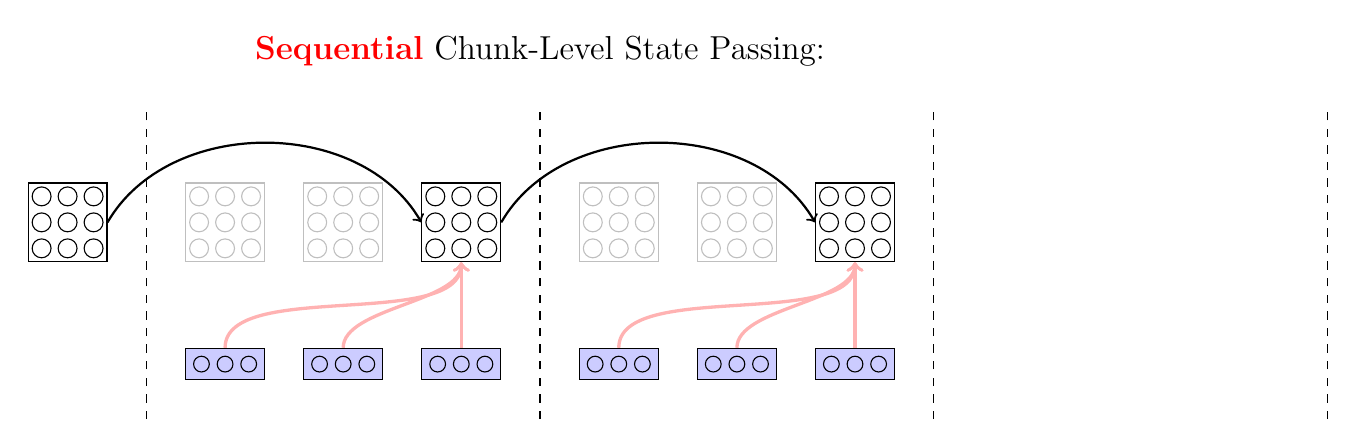
\begin{tikzpicture}
    \foreach \x in {0,5,10,15} {
        \draw[dashed] (\x,-2) -- (\x,2);
    }

        \begin{scope}[shift={(-1.5,0)}]
            \node[draw=black, minimum size=1cm] (grid-0-3) at (0.5,0.5) {};
            \foreach \x in {0,0.33,0.66} {
                \foreach \y in {0,0.33,0.66} {
                    \draw[black] (\x+0.17,\y+0.17) circle (0.12);
                }
            }
        \end{scope}

    \foreach \section [count=\i] in {0.5,5.5} {
        \foreach \offset [count=\j] in {0,1.5} {
            \begin{scope}[shift={(\section+\offset,0)}]
                \node[draw=gray!50, minimum size=1cm] (grid-\i-\j) at (0.5,0.5) {};
                \foreach \x in {0,0.33,0.66} {
                    \foreach \y in {0,0.33,0.66} {
                        \draw[gray!50] (\x+0.17,\y+0.17) circle (0.12);
                    }
                }
            \end{scope}
        }
        
        \begin{scope}[shift={(\section+3,0)}]
            \node[draw=black, minimum size=1cm] (grid-\i-3) at (0.5,0.5) {};
            \foreach \x in {0,0.33,0.66} {
                \foreach \y in {0,0.33,0.66} {
                    \draw[black] (\x+0.17,\y+0.17) circle (0.12);
                }
            }
        \end{scope}
    }
    
    \foreach \section [count=\i] in {0.5,5.5} {
        \begin{scope}[shift={(\section,-1.5)}]
            \foreach \offset [count=\j] in {0,1.5,3} {
                \node[fill=blue!20,draw=black, minimum width=1cm, minimum height=0.4cm] (rect-\i-\j) at (\offset+0.5,0.2) {};
                \foreach \x in {0.2, 0.5, 0.8} {
                    \draw[black] (\offset+\x,0.2) circle (0.1);
                }
                \draw[->,red!30,very thick] (rect-\i-\j.north) to[out=90,in=-90, looseness=0.7] 
                    ([xshift=\j*0cm]grid-\i-3.south);
            }
        \end{scope}
    }
    
% \draw[->,yellowgreen,very thick] (grid-1-3.east) to[bend left=60] node[above,font=\small,xshift=-0.5cm]{$\color{black}\boldsymbol{S}_{[2]}=\boldsymbol{S}_{[1]}{\color{yellowgreen}(\boldsymbol{I}-\boldsymbol{W}_{[2]}^\top \boldsymbol{K}_{[2]})} + {\color{red}\boldsymbol{U}_{[2]}^\top \boldsymbol{K}_{[2]}}$}  (grid-2-3.west);
\draw[->,black, thick] (grid-0-3.east)  to[bend left=60] (grid-1-3.west);
\draw[->,black, thick] (grid-1-3.east)  to[bend left=60] 
node[above,xshift=-1.5cm, yshift=0.5cm,align=center]{
  \textcolor{black}{{\large{\textbf{\color{red}Sequential}} Chunk-Level State Passing:}} \\
%   $\color{black}\boldsymbol{S}_{[i+1]}=\boldsymbol{S}_{[i]}
% + 
%     {\color{blue!50}\colorbox{red!30}{$\boldsymbol{V}_{[i]}^\top \boldsymbol{K}_{[i]}$}}$
} (grid-2-3.west);


\end{tikzpicture}

    \begin{align*}
        &\mathbf{S}_{[t+1]} = \underbrace{\mathbf{S}_{[t]}}_{\mathbb{R}^{d\times d}} + \colorbox{red!30}{$\underbrace{\color{blue!50}\mathbf{V}_{[t]}^\top}_{\mathbb{R}^{d\times C}} \underbrace{\color{blue!50}\mathbf{K}_{[t]}}_{\mathbb{R}^{C\times d}}$} &&\in \mathbb{R}^{d\times d}  \\
    \end{align*}
    Computational Complexity: $\mathcal{O}(Cd^2)$ per chunk and $\mathcal{O}(Ld^2)$ for the entire sequence.
\end{frame}

\begin{frame}{}
    
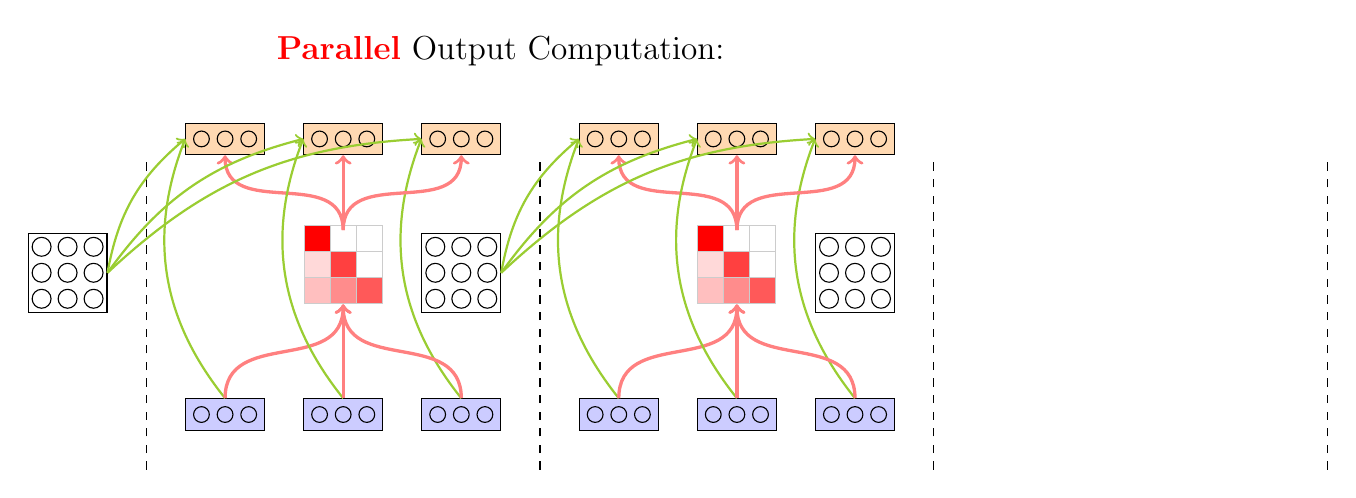
\begin{tikzpicture}[
    box/.style={
        rectangle,
        minimum size=0.5cm,
        draw=black!20
    }
]
    \foreach \x in {0,5,10,15} {
        \draw[dashed] (\x,-2) -- (\x,2);
    }
            \begin{scope}[shift={(-1.5,0)}]
            \node[draw=black, minimum size=1cm] (grid-0-3) at (0.5,0.5) {};
            \foreach \x in {0,0.33,0.66} {
                \foreach \y in {0,0.33,0.66} {
                    \draw[black] (\x+0.17,\y+0.17) circle (0.12);
                }
            }
        \end{scope}


    \foreach \section [count=\i] in {0.5,5.5} {

        % \foreach \offset [count=\j] in {0,1.5} {

     \begin{scope}[shift={(\section+1.5,0.1)}]

        \node[box, fill=red!100, minimum size=0.33cm] at (0.17,0.83) {};
        \node[box, minimum size=0.33cm] at (0.5,0.83) {};
        \node[box, minimum size=0.33cm] at (0.83,0.83) {};
        
        \node[box, fill=red!15, minimum size=0.33cm] at (0.17,0.5) {};
        \node[box, fill=red!75, minimum size=0.33cm] at (0.5,0.5) {};
        \node[box, minimum size=0.33cm] at (0.83,0.5) {};
        

        \node[box, fill=red!25, minimum size=0.33cm] at (0.17,0.17) {};
        \node[box, fill=red!45, minimum size=0.33cm] (attn-\i)at (0.5,0.17) {};
        \node[box, fill=red!65, minimum size=0.33cm] at (0.83,0.17) {};
    \end{scope}

        \begin{scope}[shift={(\section+3,0)}]
            \node[draw=black, minimum size=1cm] (grid-\i-3) at (0.5,0.5) {};
            \foreach \x in {0,0.33,0.66} {
                \foreach \y in {0,0.33,0.66} {
                    \draw[black] (\x+0.17,\y+0.17) circle (0.12);
                }
            }
        \end{scope}
    }
    

    \foreach \section [count=\i] in {0.5,5.5} {
        \begin{scope}[shift={(\section,-1.5)}]

            \foreach \offset [count=\j] in {0,1.5,3} {
                \node[draw=black, fill=blue!20, minimum width=1cm, minimum height=0.4cm] (rect-\i-\j) at (\offset+0.5,0.2) {};

                \foreach \x in {0.2, 0.5, 0.8} {
                    \draw[black] (\offset+\x,0.2) circle (0.1);
                }
                \node[draw=black, minimum width=1cm, minimum height=0.4cm,fill=orange!30] (upper-rect-\i-\j) at (\offset+0.5,0.2+3.5) {};
                \foreach \x in {0.2, 0.5, 0.8} {
                    \draw[black] (\offset+\x,0.2+3.5) circle (0.1);
                }
                
            
    \pgfmathsetmacro{\prevsection}{\i-1}
\draw[->, yellowgreen, thick] 
    (grid-\the\numexpr\i-1\relax-3.east) 
    to[bend left=20] 
    (upper-rect-\i-\j.west);

\draw[->, yellowgreen, thick] 
    (rect-\i-\j.north) 
    to[bend left=30] 
    (upper-rect-\i-\j.west);

\draw[->,red!50,very thick] (rect-\i-\j.north) to[out=90,in=-90,looseness=1.2] (attn-\i.south);

\draw[->,red!50,very thick] ([yshift=0.6cm]attn-\i.north) to[out=90,in=-90,looseness=1.2] (upper-rect-\i-\j.south);

}

\ifnum\i>1
\fi

        \end{scope}
    }
    
\node[above=0.25cm,xshift=-3cm,align=center] at (upper-rect-2-2.north) {
  \textcolor{black}{\large{\textbf{\color{red}Parallel} Output Computation:}} \\
%   ${\color{orange}\mathbf{O}_{[i]}}=\colorbox{yellowgreen!30}{${\color{blue!50}\mathbf{Q}_{[i]}}\mathbf{S}_{[i]}^\top$}+\colorbox{red!30}{\color{blue!50}$\left({\mathbf{Q}_{[i]}\mathbf{K}_{[i]}^\top \odot \mathbf{M}}\right)\mathbf{V}_{[i]}$}$
};

\end{tikzpicture}

    \vspace{-3mm}
    \begin{align*}
        {\color{orange}\mathbf{O}_{[t]}} = \colorbox{yellowgreen!30}{$\underbrace{{\color{blue!50}\mathbf{Q}_{[t]}}\mathbf{S}_{[t]}^\top}_{\text{inter-chunk}:\mathbf{O}_{[t]}^{\text{inter}}}$} + \colorbox{red!30}{$\underbrace{({\color{blue!50}\mathbf{Q}_{[t]}\mathbf{K}_{[t]}^\top \odot \mathbf{M}}){\color{blue!50}\mathbf{V}_{[t]}}}_{\text{intra-chunk}:\mathbf{O}_{[t]}^{\text{intra}}}$} \in \mathbb{R}^{C\times d}
    \end{align*}

    Computational Complexity: $\mathcal{O}(C^2d+Cd^2)$ per chunk. $\mathcal{O}(Ld^2+LCd)$ for the entire sequence.
\end{frame}
\begin{frame}{Chunkwise parallel form}
    \begin{itemize}
        \item {\textcolor{black}{Total complexity}}: $\mathcal{O}(Ld^2 + LdC)$, achieving {\textcolor{red}{subquadratic complexity}} in sequence length when $C$ is small.
        \item {\textcolor{black}{Practical settings}}: $C$ is typically set to $\{64, 128, 256\}$.
        \item {\textcolor{black}{Extensibility}}: Can be generalized to linear attention with {\textcolor{red}{decay or delta rule}} (to be discussed later).
        \item {\textcolor{black}{Adoption}}: The {\color{red}de facto standard} for {\color{red}training modern linear attention models}, including:
        \begin{itemize}
            \item {\textcolor{black}{Mamba2}}, {\textcolor{black}{Based}}, {\textcolor{black}{GLA}}, {\textcolor{black}{DeltaNet}}, {\textcolor{black}{Lightning Attention}}, {\textcolor{black}{mLSTM}}, and others.
        \end{itemize}
    \end{itemize}
\end{frame}

\begin{frame}{Flash linear attention}
    \begin{figure}
        \centering
        \includegraphics[width=.9\linewidth]{figure/fla-speed.png}
    \end{figure}
    \vspace{2mm} 
    I/O optimization significantly improves the wall-clock time.
\end{frame}

\begin{frame}{Flash linear attention}
    \begin{figure}
        \centering
        \includegraphics[width=.9\linewidth]{figure/fla-repo.png}
    \end{figure}
    The Flash Linear Attention library provides hardware-efficient implementation of various linear attention models.
    \begin{itemize}
        \item RetNet, GLA, Based, HGRN2, RWKV6, GSA, Mamba2, DeltaNet, Gated DeltaNet, RWKV7  ...
    \end{itemize}
\end{frame}

\begin{frame}{Summary}
    \begin{itemize}
        \item Linear attention = Softmax attention - softmax.
        \item Linear attention = Linear RNN + {\color{red}{matrix-valued hidden state}}.
        \item The chunkwise parallel form is more {\color{red}{hardware-friendly}} than the recurrent and parallel forms.
        \item Flash Linear Attention is an {\color{red}{I/O-aware}} implementation of the chunkwise parallel form.
    \end{itemize}
\end{frame}